\documentclass[11pt,letterpaper]{article}
\usepackage[margin=0.72in]{geometry}
\usepackage{amsmath,amssymb,tikz,array,booktabs,fancyhdr,enumitem}
\usetikzlibrary{arrows.meta}
\pagestyle{fancy}\fancyhf{}\fancyhead[L]{MATH 182: Calculus II}\fancyhead[R]{October 16, 2026}\fancyfoot[C]{\thepage}
\setlength{\headheight}{14pt}\setlength{\parindent}{0pt}\setlength{\parskip}{6pt}
\setlist[itemize]{nosep,leftmargin=*}
\newcommand{\topic}[1]{\section*{#1}}
\newcommand{\pauseq}[1]{\par\textbf{Pause and check:} #1\par}
\begin{document}
\begin{center}{\LARGE\bfseries Area and Volumes of Revolution}\\[5pt]{\large MATH 182 --- Class Notes}\\[3pt]October 16, 2026\quad$\vert$\quad 30-minute discussion\end{center}
\textbf{Objectives.} Sketch a bounded region, choose a slice direction, identify lengths and radii, and set up and evaluate area and volume integrals.

\textbf{Class sequence:} area (6 minutes), disks and washers (9 minutes), shells (9 minutes), practice and review (6 minutes).
\topic{1. Start with a slice}
An integral adds small pieces. For area, each piece is a thin rectangle. For a volume of revolution, rotate a representative slice and determine the resulting shape.
\[
\boxed{A=\int_a^b(\text{top}-\text{bottom})\,dx},\qquad
\boxed{A=\int_c^d(\text{right}-\text{left})\,dy}.
\]
\textbf{Setup routine:} sketch and shade; find intersections; draw a slice; label its lengths; write the integral with matching limits; evaluate when requested.
\topic{Example 1. Area between a line and a parabola}
Find the area enclosed by $y=x+2$ and $y=x^2$.

\textbf{Intersections:} $x^2=x+2$ gives $(x-2)(x+1)=0$, so $x=-1,2$. The line lies above the parabola on this interval.
\begin{center}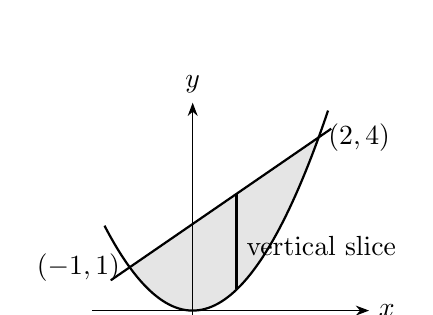
\begin{tikzpicture}[x=0.8cm,y=0.55cm,>=Stealth]
\fill[gray!20] plot[domain=-1:2,samples=60](\x,{\x+2}) -- plot[domain=2:-1,samples=60](\x,{\x*\x}) -- cycle;
\draw[->](-1.6,0)--(2.8,0)node[right]{$x$};\draw[->](0,-.3)--(0,4.8)node[above]{$y$};
\draw[thick,domain=-1.3:2.2]plot(\x,{\x+2});\draw[thick,domain=-1.4:2.15,samples=70]plot(\x,{\x*\x});
\draw[very thick](.7,.49)--(.7,2.7);\node[right]at(.7,1.5){vertical slice};
\node[left]at(-1,1){$(-1,1)$};\node[right]at(2,4){$(2,4)$};
\end{tikzpicture}\end{center}
The slice has height $(x+2)-x^2$ and thickness $dx$. Therefore
\[
A=\int_{-1}^2(x+2-x^2)\,dx
=\left[\frac{x^2}{2}+2x-\frac{x^3}{3}\right]_{-1}^2
=\boxed{\frac92\text{ square units}}.
\]
\textbf{Check your understanding.} Why must we subtract the parabola from the line? Because a slice length is top minus bottom and must be nonnegative.
\newpage
\topic{2. Disks and washers: perpendicular slices}
A slice perpendicular to the rotation axis sweeps out a disk or washer. The outer radius $R$ and inner radius $r$ are distances from the axis.
\[
\boxed{V=\pi\int(R^2-r^2)\,dt},\qquad
\text{disk: }r=0,\quad dt=dx\text{ or }dy.
\]
\textbf{Axis guide.} About a horizontal axis, use vertical slices ($dx$). About a vertical axis, use horizontal slices ($dy$).
\topic{Example 2. Disk method}
Rotate the region under $y=\sqrt{4-x}$, above the $x$-axis, for $0\leq x\leq4$, about the $x$-axis.

A vertical slice touches the rotation axis, so it creates a disk. Its radius is $R(x)=\sqrt{4-x}$.
\begin{align*}
V&=\pi\int_0^4\left(\sqrt{4-x}\right)^2\,dx
=\pi\int_0^4(4-x)\,dx\\
 &=\pi\left[4x-\frac{x^2}{2}\right]_0^4
=\boxed{8\pi\text{ cubic units}}.
\end{align*}
\topic{Example 3. Washer method}
Rotate the region between $y=x+1$ and $y=1$, for $0\leq x\leq2$, about the $x$-axis.

The slice does not reach the axis, so there is a hole. The outer radius is $R=x+1$; the inner radius is $r=1$.
\begin{align*}
V&=\pi\int_0^2\big[(x+1)^2-1^2\big]\,dx\\
 &=\pi\int_0^2(x^2+2x)\,dx
=\pi\left[\frac{x^3}{3}+x^2\right]_0^2
=\boxed{\frac{20\pi}{3}\text{ cubic units}}.
\end{align*}
\textbf{Essential distinction:} subtract the areas of two disks:
\[\pi R^2-\pi r^2=\pi(R^2-r^2),\qquad\text{not }\pi(R-r)^2.\]
\topic{Quick extension: a shifted axis}
If Example 3 is rotated about $y=-2$, measure each distance from that line:
\[R=(x+1)-(-2)=x+3,\qquad r=1-(-2)=3.\]
The setup becomes
\[\boxed{V=\pi\int_0^2[(x+3)^2-3^2]\,dx}.\]
\textbf{Key question:} Which boundary is farther from the actual axis? That boundary determines the outer radius.
\newpage
\topic{3. Cylindrical shells: parallel slices}
A slice parallel to the rotation axis sweeps out a thin cylindrical shell. Unrolling it gives a rectangle with length equal to its circumference.
\[
\boxed{dV=2\pi(\text{radius})(\text{height})(\text{thickness})}.
\]
The shell height is the length of the original slice. For a horizontal slice, this is a horizontal length.
\topic{Example 4. Horizontal shells about the $x$-axis}
Rotate the first-quadrant region bounded by $x=y^2$, $x=4$, and $y=0$ about the $x$-axis. Use shells.

\textbf{Bounds:} $y^2=4$ gives the upper height $y=2$. Thus $0\leq y\leq2$.

\textbf{One horizontal slice:}
\[
\text{radius}=y,\qquad
\text{height}=\text{right}-\text{left}=4-y^2,\qquad
\text{thickness}=dy.
\]
\begin{center}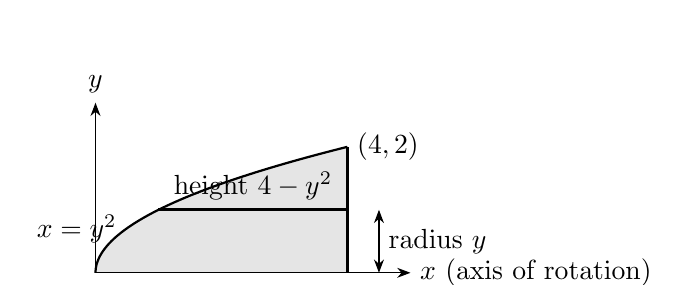
\begin{tikzpicture}[x=.8cm,y=.8cm,>=Stealth]
\fill[gray!20] (0,0)--(4,0)--(4,2)--plot[domain=2:0,samples=60]({\x*\x},\x)--cycle;
\draw[->](0,0)--(5,0)node[right]{$x$ (axis of rotation)};
\draw[->](0,0)--(0,2.7)node[above]{$y$};
\draw[thick,domain=0:2,samples=60]plot({\x*\x},\x);
\draw[thick](4,0)--(4,2);\draw[very thick](1,1)--(4,1);
\draw[<->](4.5,0)--(4.5,1)node[midway,right]{radius $y$};
\node[above]at(2.5,1){height $4-y^2$};
\node[right]at(4,2){$(4,2)$};\node[left]at(.49,.7){$x=y^2$};
\end{tikzpicture}\end{center}
Therefore
\begin{align*}
V&=2\pi\int_0^2y(4-y^2)\,dy\\
 &=2\pi\left[2y^2-\frac{y^4}{4}\right]_0^2
=2\pi(8-4)=\boxed{8\pi\text{ cubic units}}.
\end{align*}
\textbf{Independent check:} vertical disks have radius $\sqrt{x}$ for $0\leq x\leq4$, so $V=\pi\int_0^4x\,dx=8\pi$.
\topic{Choose the direction before writing a formula}
\begin{center}\begin{tabular}{lll}\toprule
Axis & Vertical slices ($dx$) & Horizontal slices ($dy$)\\\midrule
Horizontal & Disks/washers & Shells\\
Vertical & Shells & Disks/washers\\\bottomrule
\end{tabular}\end{center}
\textbf{Vertical-shell model:} about the $y$-axis, a region with top $f(x)$ and bottom $g(x)$, contained in $x\geq0$, has
\[V=2\pi\int_a^b x[f(x)-g(x)]\,dx.\]
\newpage
\topic{4. Practice and final checks}
\textbf{Practice A --- washer setup.} Rotate the region between $y=3$ and $y=x$, for $0\leq x\leq3$, about the $x$-axis. Label $R$ and $r$, then set up the volume integral.
\par\vspace{0.55in}
\textbf{Practice B --- shell setup.} Rotate the region under $y=4-x$ and above $y=0$, for $0\leq x\leq4$, about the $y$-axis. Label the shell radius and height, then set up the volume integral.
\par\vspace{0.55in}
\topic{Answer checks}
\textbf{A:} $R=3$, $r=x$, and
\[V=\pi\int_0^3(9-x^2)\,dx=\boxed{18\pi}.\]
\textbf{B:} radius $x$, height $4-x$, and
\[V=2\pi\int_0^4x(4-x)\,dx=\boxed{\frac{64\pi}{3}}.\]
\topic{Before submitting a solution}
\begin{itemize}
\item Does the sketch show the bounded region and the actual rotation axis?
\item Are the slice lengths and radii nonnegative?
\item Do the limits match the integration variable?
\item For washers, did you use $R^2-r^2$? For shells, did you use $2\pi rh$?
\item Does a boundary change inside the interval? If so, split the integral where its formula changes, or choose another slice direction.
\item Have you used the requested method and kept the answer exact?
\end{itemize}
\topic{Exit question}
For rotation about the $y$-axis, explain why a vertical slice produces a shell and a horizontal slice produces a washer.

\textit{Explanation:} the vertical slice is parallel to the axis and sweeps around it at a fixed radius, forming a shell. The horizontal slice is perpendicular to the axis and sweeps out a circular cross-section, forming a disk or washer.
\end{document}
